% Editable report draft. Compile from this folder, leaving ../figures unchanged.
% pdflatex -jobname=DT081A_Lab3_Report_Jakob_Obid_DRAFT main.tex
\documentclass[11pt,a4paper]{article}
\usepackage[T1]{fontenc}
\usepackage{lmodern}
\usepackage[utf8]{inputenc}
\usepackage[margin=22mm]{geometry}
\usepackage{graphicx}
\usepackage{amsmath}
\usepackage{booktabs}
\usepackage[font=small,labelfont=bf]{caption}
\usepackage{placeins}
\usepackage{float}
\usepackage{pdflscape}
\usepackage[hidelinks]{hyperref}
\graphicspath{{../figures/}}
\setlength{\parindent}{0pt}
\setlength{\parskip}{5pt}
\setlength{\emergencystretch}{3em}
\setlength{\textfloatsep}{12pt}
\setlength{\intextsep}{10pt}
\setlength{\abovecaptionskip}{5pt}
\setlength{\belowcaptionskip}{0pt}
\renewcommand{\arraystretch}{1.15}
\renewcommand{\topfraction}{0.95}
\renewcommand{\bottomfraction}{0.95}
\renewcommand{\textfraction}{0.04}
\renewcommand{\floatpagefraction}{0.8}
\setcounter{topnumber}{4}
\setcounter{bottomnumber}{4}
\setcounter{totalnumber}{6}
\raggedbottom
\widowpenalty=10000
\clubpenalty=10000
\brokenpenalty=10000
\hypersetup{pdftitle={DT081A Lab 3 Report Draft},pdfauthor={Yacoub Dawli and Obid Alrhman Aljabi}}
\newcommand{\question}[1]{\par\smallskip\noindent\textbf{Question #1.}\ }
\newcommand{\reportfigure}[4][\linewidth]{%
\begin{figure}[H]\centering
\includegraphics[width=#1]{#2}
\caption{#3}\label{#4}
\end{figure}}
\begin{document}
\begin{center}
{\Large DT081A --- Signal and Image Processing\par}
\vspace{3pt}
{\Large Lab 3 Report\par}
\vspace{5pt}
Group members:\par
Yacoub Dawli (Jakob) --- \texttt{yada2100@student.miun.se}\par
Obid Alrhman Aljabi --- \texttt{obal2302@student.miun.se}\par
24 October 2026\par
\small Draft for review
\end{center}
\vspace{-3pt}

\section{Introduction}
In this lab, we studied pixel transforms, colour reduction, filtering, the Fourier transform, histograms and morphology. We compared changes in detail, contrast and noise using images and numerical results. We also measured execution time and calculated memory needs.

\section{Experimental Setup}
We used Python with NumPy, OpenCV and Matplotlib. Our source was the course image \texttt{peppers.tiff} ($512\times512$ pixels). The suggested \texttt{ManWoman.png} was unavailable. The instructions allow other images, and peppers has useful colour boundaries and shading.

OpenCV loads colour images in BGR order. We converted to RGB for colour display and used a grayscale copy for most other tasks. Original intensities were stored as 8-bit integers. We used floating-point values where calculations could go below 0 or above 255. We also used small synthetic images for Sections 7 and 11. The settings are given with each result. Recorded timings used \texttt{time.time()} and OpenCV 5.0.0; they describe one run on our computer.

\section{Results and Analysis}
The question numbers below match Lab 3, Version 1.1. Figures show the saved experimental results.

\subsection{Gamma Correction}
\question{1.1}
We implemented the normalized power law
$ I_{\mathrm{out}}=255(I_{\mathrm{in}}/255)^\gamma $.
Table~\ref{tab:gamma} shows the three test values for $\gamma=2.0$.
All become darker because raising a value between 0 and 1 to a power above 1 makes it smaller. Converting to \texttt{uint8} removes the decimal part.

\begin{table}[!htbp]\centering
\caption{Gamma calculation with $\gamma=2.0$.}\label{tab:gamma}
\begin{tabular}{rrr}\toprule
Input & Before integer conversion & Output as \texttt{uint8}\\\midrule
64 & 16.063 & 16\\
128 & 64.251 & 64\\
192 & 144.565 & 144\\\bottomrule
\end{tabular}
\end{table}

\question{1.2}
With $\gamma=2.2$, the grayscale image became darker and the mean intensity fell from 120.22 to 61.00 (Figure~\ref{fig:gamma}). The histogram moved towards lower values. Dark values were packed closer together, and integer conversion left gaps at some output levels. Gamma changes brightness nonlinearly. This relates to the eye's unequal sensitivity to brightness changes, although a power curve is not an exact logarithmic model of vision. We used the lab's exponent $\gamma$, rather than the inverse exponent used for camera pre-correction.

\reportfigure{section1_gamma_histograms.png}{Original and gamma-corrected images and histograms. Both images use 0--255; histogram axes are shared.}{fig:gamma}
\FloatBarrier

\subsection{Colorspaces}
\question{2.1}
We converted the original image to YCrCb and extracted channels in OpenCV's order: Y, Cr, Cb. Brightness is approximately $Y=0.299R+0.587G+0.114B$.
Table~\ref{tab:spread} compares the spread of Y and RGB values. Standard deviation describes how spread out the values are. G had the largest spread. Y was less spread out than G, but more than R and B. R had many high values, while B had mostly low values.

\begin{table}[!htbp]\centering
\caption{Intensity spread in the original image.}\label{tab:spread}
\begin{tabular}{lrrr}\toprule
Channel & Minimum & Maximum & Standard deviation\\\midrule
Y & 0 & 228 & 53.88\\
R & 0 & 231 & 45.17\\
G & 0 & 237 & 75.05\\
B & 0 & 229 & 44.29\\\bottomrule
\end{tabular}
\end{table}

Y describes brightness, so it is useful for detecting rapid brightness changes in one channel. Boundaries between colours with similar brightness can still be missed.

\question{2.2}
We kept Y unchanged and divided both the width and height of Cb and Cr by each factor. We used area interpolation to reduce them and linear interpolation to restore their size for display. For $N$ pixels, factor 2 changes the sample count from $3N$ to $N+N/4+N/4=1.5N$, saving 50\%. Here that is 786,432 to 393,216 bytes. Factors 4 and 8 need 294,912 and 270,336 bytes, saving 62.5\% and 65.625\%. These are reduced channel sizes before reconstruction, not compressed file sizes.

Factor 2 looked close to the original. At factor 4, colour boundaries became softer. Factor 8 showed clearer colour blending at the yellow-green and red pepper boundary (Figure~\ref{fig:chroma}). Brightness detail remained because Y was kept. Visibility also depends on the viewing size.

\reportfigure{section2_chroma_subsampling.png}{Chroma subsampling with Y unchanged. The lower row enlarges the same $128\times128$ crop in each image.}{fig:chroma}
\FloatBarrier

\subsection{Quantization and Sampling}
\question{3.1}
We divided each RGB channel by 16 using integer division. This gives 16 possible 4-bit levels. Multiplying the level numbers by 16 for display gives $0,16,\ldots,240$, following the teacher's lower-value convention. The image used 15 levels per channel because no original channel values reached 240. Shapes stayed clear, but smooth colour changes looked slightly stepped and darker (Figure~\ref{fig:4bit}).

The theoretical compression ratio is $8/4=2{:}1$, or 50\% saving. Packed 4-bit storage would use 393,216 bytes instead of 786,432. Our quantized NumPy array still used \texttt{uint8}, so its actual size remained 786,432 bytes.

\reportfigure[0.90\linewidth]{section3_4bit_quantization.png}{Original RGB image and 4-bit quantization. Each channel has 16 possible levels.}{fig:4bit}

\question{3.2}
For grayscale, division by 32 gave eight 3-bit levels, displayed as $0,32,\ldots,224$. Each new bar combines 32 original intensity values. All eight levels were occupied; the last had only 29 pixels (Figure~\ref{fig:3bit}). Both histograms count 262,144 pixels, with axes showing original intensities and quantized level numbers. Nearby intensities became identical, causing banding and loss of shading and texture. Outlines remained clear.

\reportfigure[0.85\linewidth]{section3_3bit_histograms.png}{Original grayscale and 3-bit images with their histograms. Quantization groups many original values into eight levels.}{fig:3bit}
\FloatBarrier

\subsection{Convolution and Edge Detection}
\question{4.1}
We formed a 2D Gaussian kernel from a 1D kernel, using $\sigma=1.0$. We compared \texttt{filter2D()} and \texttt{sepFilter2D()} with float64 output and reflected borders (\texttt{BORDER\_REFLECT\_101}). After one warm-up call per method, we averaged 30 calls. Kernel creation and plotting were outside the timing. Table~\ref{tab:gaussian} gives the recorded results.

\begin{table}[!htbp]\centering
\caption{Average Gaussian filtering time per image.}\label{tab:gaussian}
\begin{tabular}{lrr}\toprule
Kernel & Ordinary 2D (ms) & Separable (ms)\\\midrule
$5\times5$ & 5.420 & 1.429\\
$11\times11$ & 9.880 & 10.455\\
$21\times21$ & 23.481 & 24.022\\\bottomrule
\end{tabular}
\end{table}

Separable filtering was clearly faster for $5\times5$. The other times were close, with ordinary 2D slightly faster. A direct kernel uses $k^2$ weights per pixel, while two separable passes use about $2k$. This can help for large kernels and images, but actual speed also depends on the implementation. Our run does not show that separable filtering is always faster. Both methods gave the same visible blur; their largest difference was about 0.000002 intensity units. Timings can vary between runs.

\question{4.2}
Our \texttt{detect\_horizontal\_edges()} function uses a $3\times3$ Sobel filter with \texttt{dx=0, dy=1}. It measures brightness changes from top to bottom, which highlights horizontal boundaries. We displayed absolute values. Top and bottom pepper boundaries were strong, while long vertical sides were weaker (Figure~\ref{fig:sobel}). The \texttt{dx=1, dy=0} comparison highlights vertical edges. Curved or sloping edges can appear in both.

\reportfigure{section4_sobel_edges.png}{Sobel derivatives. The horizontal and vertical edge displays use the same strength scale.}{fig:sobel}

\question{4.3}
We combined the signed derivatives as
$G=\sqrt{G_x^2+G_y^2}$ and normalized a copy to 0--255 for display.
The magnitude shows more complete pepper outlines and stems because it includes changes in both directions. Brighter pixels indicate stronger edges. The right panel of Figure~\ref{fig:morph} shows this result, reused in the morphological comparison.

\FloatBarrier

\subsection{Matrix Operations}
\question{5.1}
We stacked the grayscale pixels into one column, applied
$1.2(I-128)+128+20$, clipped to 0--255 and reshaped the result. A second version used nested Python loops with the same formula. Over five runs, NumPy averaged 2.040 ms and the loops 468.915 ms. NumPy was 229.82 times faster using unrounded times. Timings include calculation, output creation and type conversion; loading and plotting were excluded.

Both methods gave exactly the same image. It looked brighter overall, with some highlights clipped at 255. NumPy handles the array work inside its library, avoiding a Python loop for every pixel.

\question{5.2}
The stacked $512\times512$ image has 262,144 values. The full convolution matrix H therefore has $262,144\times262,144=68,719,476,736$ elements. It needs 274,877,906,944 bytes (256 GiB) as float32, or 549,755,813,888 bytes (512 GiB) as float64. GiB uses $1024^3$ bytes.

We calculated these sizes without allocating H. Most entries would be zero for a $3\times3$ convolution. Storing nine kernel weights and applying them to local neighbourhoods is much more practical.

\subsection{Pixel-Based Processing}
\question{6.1}
We compared direct NumPy evaluation of our logarithmic transform with a 256-entry lookup table. After warm-up, we averaged 30 applications per method. Direct computation took 9.469 ms per image and lookup took 2.468 ms: lookup was 3.84 times faster. Table creation took a separate 0.539 ms and was excluded from the application timing. It can be reused while the transform stays the same.

The lookup avoids calculating logarithms for every pixel. Both methods gave identical \texttt{uint8} results, with values from 0 to 240.

\question{6.2}
We used two matching logarithmic halves joined at intensity 127.5, with strength 4. The curve in Figure~\ref{fig:log} is steeper in the middle and flatter at the ends. Equal input gaps of 32 units gave output gaps of 17 for 0--32, 64 for 112--144, and 18 for 223--255. Middle differences were enlarged, while shadow and highlight differences were compressed. The full curve maps 0 to 0 and 255 to 255 without reversing intensity order.

Dark gaps looked darker and lighter areas looked brighter. Middle shading was more strongly separated, while small differences near the ends had less contrast.

\reportfigure{section6_log_transformation.png}{Logarithmic contrast transformation, strength 4, and its transfer curve. The dashed line leaves intensities unchanged.}{fig:log}
\FloatBarrier

\subsection{Elementary Images}
\question{7.1}
We used the teacher's ramp, step and sine vectors with size 16. Each outer product combines a row pattern with a column pattern (Figure~\ref{fig:elementary}). Ramp $\times$ Ramp changes smoothly downwards and to the right. Step $\times$ Ramp has a horizontal boundary and a gradual change across the lower half. Step $\times$ Step creates a lower-right block with sharp boundaries. Step $\times$ Sine adds repeating bright and dark columns in the lower half. Ramps describe smooth changes, steps sharp boundaries, and sines repeated changes. The shared scale is $-1$ to 1, so zero appears middle gray.

\reportfigure[0.90\linewidth]{section7_elementary_images.png}{Four $16\times16$ outer products with a shared scale, including negative sine values.}{fig:elementary}

\question{7.2}
Our target was an $8\times8$ white square in a $16\times16$ black image: rows 8--15 and columns 4--11, counting from zero. We fitted Step $\times$ Ramp, Step $\times$ Step and Step $\times$ Sine using \texttt{np.linalg.lstsq()}. This finds the smallest sum of squared pixel errors for these three images. Table~\ref{tab:weights} gives the weights.

\begin{table}[!htbp]\centering
\caption{Weights for the three-image square approximation.}\label{tab:weights}
\begin{tabular}{lr}\toprule
Elementary image & Weight\\\midrule
Step $\times$ Ramp & 0.156058\\
Step $\times$ Step & 0.812731\\
Step $\times$ Sine & 0.688038\\\bottomrule
\end{tabular}
\end{table}

The mean squared error (MSE) was 0.107400 on the 0--1 scale. This is the average squared pixel difference; zero would mean an exact match. The unclipped approximation ranged from 0.000000 to 0.895961. Its upper half stayed black and its horizontal boundary was correct, but the square's interior was uneven and the side boundaries were inaccurate. Gray bands remained outside the square (Figure~\ref{fig:shape}). These three patterns could only give a coarse approximation.

\reportfigure{section7_shape_approximation.png}{Target square, raw three-image approximation and absolute pixel error, all on the 0--1 scale.}{fig:shape}
\FloatBarrier

\subsection{Transforms and Frequency Domain}
\question{8.1}
We applied \texttt{fft2()} to the original grayscale image, moved zero frequency to the centre with \texttt{fftshift()}, and displayed \texttt{log1p(abs(fshift))}. The bright centre contains the average brightness and strong slow changes. Faster changes, including edges, contribute farther from the centre (Figure~\ref{fig:fft}).

Horizontal and vertical streaks pass through the centre, with weaker patterns farther out. Vertical edges change brightness across columns and contribute along the horizontal frequency direction; horizontal edges contribute along the vertical direction. Image borders also affect the streaks. Curved edges contribute several directions and frequencies. The spectrum does not show edge positions, so we cannot assign a particular peak to one pepper edge.

\reportfigure{section8_fft_spectrum.png}{Original image and logarithmic FFT magnitude. Axes show frequency bins relative to the centre.}{fig:fft}

\question{8.2}
We used the teacher's circular low-pass mask with radius less than 40 frequency bins in the $512\times512$ FFT grid. After multiplication, \texttt{ifftshift()} and \texttt{ifft2()} returned the filtered image. We kept its real part. The main shapes and broad shading remained, but small surface and stem details became weaker. Edges became softer (Figure~\ref{fig:frequency}). Some bright and dark ripples, called ringing, appeared near strong boundaries because the cutoff was sharp.

Raw values were $-17.078$ to 243.781. Negatives display as black; the data were kept.

\question{8.3}
We followed the hint and calculated \texttt{highpass = original - lowpass} in floating point. This keeps the complementary high-frequency content. Outlines, stems and fine details stood out, while smooth areas were near zero. Ringing was also visible. The signed range was $-155.400$ to 113.396. We displayed symmetric limits of about $\pm155.400$, with zero as middle gray, positive differences lighter and negative differences darker.

Adding the unchanged low-pass and high-pass arrays recovered the original with maximum pixel error 0. The maximum imaginary part after inverse FFT was $6.172\times10^{-14}$.

\reportfigure{section8_frequency_filtering.png}{Original and low-pass images use 0--255. High-pass middle gray represents zero difference, not ordinary image brightness.}{fig:frequency}
\FloatBarrier

\subsection{Histograms and Image Enhancement}
\question{9.1}
We normalized the grayscale histogram so its bars sum to 1. About 76.43\% of pixels were in the range 64--191. The highest bar was at 96, with another broad lighter group around 150--190 (Figure~\ref{fig:hist}). Most pixels were in the middle range, and few were very bright. The maximum was 228. A histogram shows how common values are, but not where the pixels occur.

The cumulative histogram gives the proportion at or below each intensity. It was 52.51\% at 127 and 92.19\% at 191. It rises fastest where many pixels occur and reaches 1 at 228. We used the interval \texttt{[0,256]} instead of the example's \texttt{[0,255]}, because OpenCV excludes the upper limit and all 256 levels should be included.

\reportfigure{section9_histograms.png}{Original normalized histogram and cumulative histogram.}{fig:hist}

\question{9.2}
We reduced contrast with $128+0.5(I-128)$, using floating point before clipping and integer conversion. The range shrank from 0--228 to 64--178, making the image flatter. We then used the reduced image's cumulative histogram to create a lookup table: $T(r)=255\,\mathrm{CDF}(r)$, converted to \texttt{uint8}.

Our equalized result and \texttt{cv2.equalizeHist()} both used 0--255. Compared with the low-contrast image, shading, stems and surface details became clearer. Compared with the original, gaps looked darker and highlights brighter; some fine grain also became clearer (Figure~\ref{fig:equalization}).

The two equalized results looked almost identical. Their maximum absolute difference was 1 intensity level and their mean absolute difference was 0.443756. OpenCV subtracts the first nonzero cumulative value, stretches the remaining range and rounds. Our method follows the teacher's formula and drops fractional parts. This explains the small difference.

\reportfigure[0.90\linewidth]{section9_histogram_equalization.png}{Original, reduced-contrast and equalized images. Our result is compared with OpenCV on the same 0--255 display scale.}{fig:equalization}
\FloatBarrier

\clearpage
\subsection{Noise and Noise Reduction}
\question{10.1}
We measured PSNR against the clean grayscale image using \texttt{cv2.PSNR()}. Higher PSNR means smaller overall pixel errors. We used random seed 42 and one mean-zero Gaussian sample, scaled to noise standard deviation $\sigma=25$ or 35. Noise was added in floating point, then clipped and converted to \texttt{uint8}. This avoids the wraparound possible in the teacher's early integer conversion.

The filters stayed fixed: median $3\times3$, and bilateral diameter 9, \texttt{sigmaColor=75}, \texttt{sigmaSpace=75}. Bilateral trials at noise $\sigma=25,30,35$ gave 28.860, 28.004 and 26.888 dB. We chose 35 for the close match in Table~\ref{tab:match}. The output gap was 0.059 dB. Since the inputs had different noise strengths, this does not rank the filters on the same input.

\begin{table}[!htbp]\centering
\caption{Different Gaussian noise strengths giving similar filtered PSNR.}\label{tab:match}
\begin{tabular}{lrrr}\toprule
Filter & Noise $\sigma$ & Input (dB) & Output (dB)\\\midrule
Median, $3\times3$ & 25 & 20.318 & 26.829\\
Bilateral, 9, 75, 75 & 35 & 17.519 & 26.888\\\bottomrule
\end{tabular}
\end{table}

Both results had less grain. The median image still looked grainy, while the bilateral image was smoother with softer stem detail and boundaries. Similar PSNR did not mean identical appearance.

\question{10.2}
For a direct comparison, both filters received the same noisy input for each noise type. We used $3\times3$ mean and median filters. Gaussian noise reused $\sigma=25$. Salt-and-pepper noise used 4\% total probability: 2\% black and 2\% white, without overlap. The seeded run selected 3.986\% of pixels.

\begin{table}[!htbp]\centering
\caption{Mean and median filtering, using the clean image as reference.}\label{tab:noise}
\begin{tabular}{lrrrr}\toprule
Noise & Input & Mean & Median & Mean $-$ Median\\
 & \multicolumn{4}{c}{PSNR or PSNR difference (dB)}\\\midrule
Gaussian, $\sigma=25$ & 20.318 & 27.237 & 26.829 & $+0.409$\\
Salt-and-pepper, 4\% & 19.296 & 26.516 & 34.035 & $-7.519$\\\bottomrule
\end{tabular}
\end{table}

Mean filtering was higher by 0.409 dB for Gaussian noise (Table~\ref{tab:noise}). Averaging reduced the scattered noise but also blurred edges. Median filtering was higher by 7.519 dB for salt-and-pepper noise. It removed many isolated extreme pixels, while the mean spread them into visible gray marks and blur. Differences were calculated before rounding. Figure~\ref{fig:noise} shows these effects; some fine details were softened even in the median result.
\FloatBarrier
\begin{landscape}
\begin{figure}[p]\centering
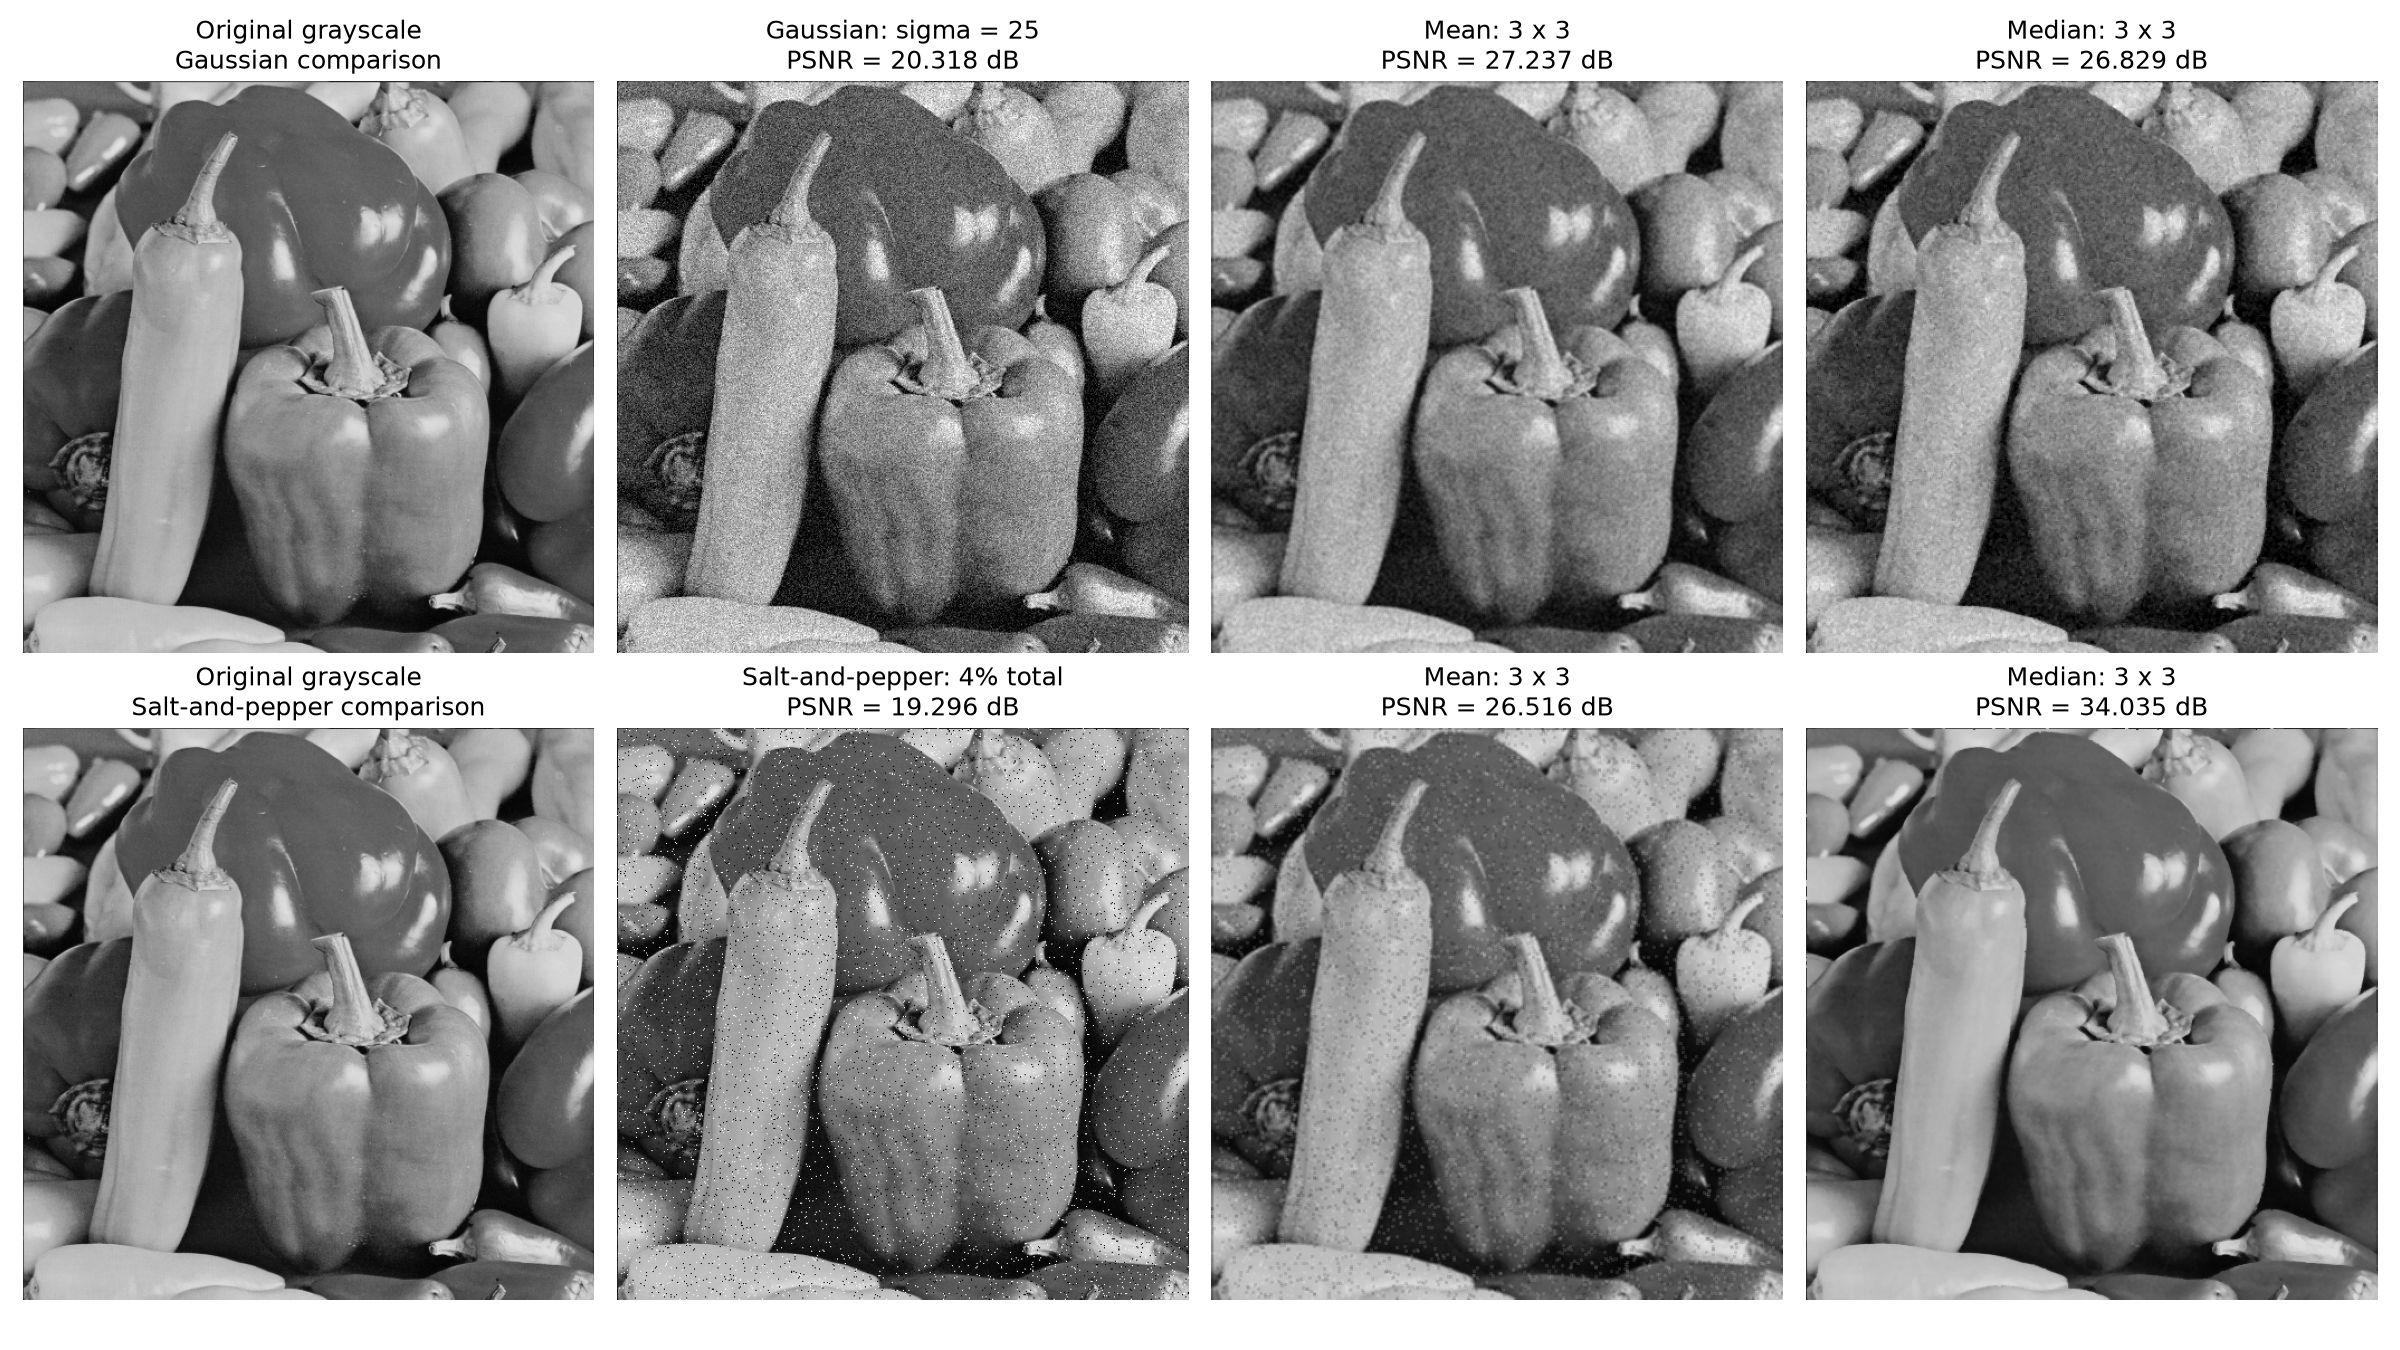
\includegraphics[width=0.97\linewidth]{section10_mean_median_comparison.png}
\caption{Mean and median filtering with $3\times3$ kernels. Gaussian noise is above and salt-and-pepper noise below. Each row uses the same noisy input for both filters. All panels use 0--255.}
\label{fig:noise}
\end{figure}
\end{landscape}

\subsection{Morphological Filtering}
\question{11.1}
We made two $128\times128$ binary test images, with white objects on black backgrounds. Test A had a circle, rectangle and triangle. Test B had two differently sized circles, a rectangle and a triangle. Each also had three isolated white pixels and a $2\times2$ black hole.

We first applied opening (erosion then dilation) with the teacher's $3\times3$ cross to remove the specks. Closing (dilation then erosion) with a $5\times5$ elliptical kernel filled the hole. We then counted 8-connected white regions using \texttt{connectedComponents()} and subtracted one for the background. Test A gave 3 objects and Test B gave 4, matching both expected counts (Figure~\ref{fig:objects}). Some corners became rounder. Touching objects would count together, so the method depends on separated objects.

\reportfigure[0.96\linewidth]{section11_object_counting.png}{Binary tests before cleaning, after opening, and after closing with object counts. The same sequence was used for both tests.}{fig:objects}

\question{11.2}
We calculated the morphological gradient as dilation minus erosion using the $3\times3$ cross, and compared it with Section 4's Sobel magnitude. Both showed pepper outlines, stems and weaker texture (Figure~\ref{fig:morph}). The morphological result showed more fine grain on some surfaces, while Sobel outlines looked smoother.

The raw ranges were 0--204 for morphology and 0--812.857 for Sobel. Each display was separately normalized to 0--255, so displayed brightness cannot be compared as raw gradient strength. Morphology is useful for binary shapes and their boundaries; the kernel affects edge appearance and thickness. Sobel is useful for grayscale brightness changes. Its separate derivatives help when direction matters, although the displayed magnitude combines strength without showing direction.

\reportfigure{section11_gradient_comparison.png}{Original, morphological gradient and reused Sobel magnitude. Both gradient displays are separately normalized.}{fig:morph}
\FloatBarrier

\section{Discussion}
The experiments showed several useful tradeoffs. Vector operations and lookup tables saved time while giving exactly the same outputs as their comparison methods. Separability reduces the number of kernel calculations, but our measured Gaussian times also depended on the library routines and kernel size. A single timing run cannot establish a general speed ranking.

Low-pass filtering removed detail and softened edges. The sharp frequency cutoff also caused ringing. Histogram equalization spread brightness values and made details clearer, but also showed more grain. A filter's effect depended on the noise: mean filtering was slightly better for our Gaussian setting, while median filtering was much better for salt-and-pepper noise.

The shape experiments also had limits. Three elementary images could only approximate the square. Morphological cleaning worked for our separated binary objects, but touching shapes could count as one. These results depend on the chosen image and settings.

\section{Conclusion}
We learned how pixel transforms, colour reduction and filtering change image brightness, detail and noise. Numerical comparisons helped us check what we saw in the figures. We also saw why practical choices matter: the right filter depends on the task, and a simpler representation can save time or memory while losing some information.

\clearpage
\section*{Appendix: Code Snippets}
These excerpts are from \texttt{labbs/lab3/lab3.py}. The full script contains the setup and remaining experiments. The methods follow Lab 3, Version 1.1; the report structure follows the course report template.

\subsection*{Gamma correction}
\begin{samepage}
\begin{small}
\begin{verbatim}
def apply_gama(image, gamma):
    # Use the lab's exponent gamma on intensities between 0 and 1.
    image_float = image.astype(np.float32) / 255.0
    corrected_image = 255.0 * np.power(image_float, gamma)
    return np.uint8(corrected_image)
\end{verbatim}
\end{small}
The input is normalized, raised to the chosen power and converted back to 8-bit intensities.
\end{samepage}

\subsection*{FFT filtering}
\begin{samepage}
\begin{small}
\begin{verbatim}
filtered_fft = fshift * lowpass_mask
lowpass_complex = np.fft.ifft2(np.fft.ifftshift(filtered_fft))
lowpass = lowpass_complex.real

# Section 8.3: subtract the smooth image, keeping positive and negative values.
highpass = gray.astype(np.float64) - lowpass
\end{verbatim}
\end{small}
The previously created circular mask keeps frequencies within 40 bins of the centre. The inverse FFT gives the smooth image. Subtraction keeps the remaining signed detail.
\end{samepage}

\subsection*{Histogram equalization}
\begin{samepage}
\begin{small}
\begin{verbatim}
low_hist = cv2.calcHist([low_contrast], [0], None, [256], [0, 256]).ravel()
low_hist = low_hist.astype(np.float64) / low_hist.sum()
low_cumulative_hist = np.cumsum(low_hist)
equalization_table = (255 * low_cumulative_hist).astype(np.uint8)
equalized = equalization_table[low_contrast]
\end{verbatim}
\end{small}
The cumulative probabilities create a lookup table, which maps the reduced-contrast pixels to new intensities.
\end{samepage}

\subsection*{Morphological object counting}
\begin{samepage}
\begin{small}
\begin{verbatim}
    opened = cv2.morphologyEx(binary_images[i], cv2.MORPH_OPEN, cross_kernel)
    cleaned = cv2.morphologyEx(opened, cv2.MORPH_CLOSE, disk_kernel)
    num_labels, labels = cv2.connectedComponents(cleaned, connectivity=8)
    object_count = num_labels - 1  # Exclude the black background.
\end{verbatim}
\end{small}
Inside the loop over both binary images, opening removes isolated specks, closing fills the small hole, and counting labels excludes the background.
\end{samepage}

\end{document}
